\let\negmedspace\undefined
\let\negthickspace\undefined
\documentclass[article]{IEEEtran}
       \def\inputGnumericTable{}                                 %%
\usepackage{cite}
\usepackage{amsmath,amssymb,amsfonts,amsthm}
\usepackage{algorithmic}
\usepackage{graphicx}
\usepackage{textcomp}
\usepackage{xcolor}
\usepackage{txfonts}
\usepackage{listings}
\usepackage{enumitem}
\usepackage{mathtools}
\usepackage{gensymb}
\usepackage[breaklinks=true]{hyperref}
\usepackage{tkz-euclide} % loads  TikZ and tkz-base
\usepackage{listings}
%
%\usepackage{setspace}
%\usepackage{gensymb}
%\doublespacing
%\singlespacing

%\usepackage{graphicx}
%\usepackage{amssymb}
%\usepackage{relsize}
%\usepackage[cmex10]{amsmath}
%\usepackage{amsthm}
%\interdisplaylinepenalty=2500
%\savesymbol{iint}
%\usepackage{txfonts}
%\restoresymbol{TXF}{iint}
%\usepackage{wasysym}
%\usepackage{amsthm}
%\usepackage{iithtlc}
%\usepackage{mathrsfs}
%\usepackage{txfonts}
%\usepackage{stfloats}
%\usepackage{bm}
%\usepackage{cite}
%\usepackage{cases}
%\usepackage{subfig}
%\usepackage{xtab}
%\usepackage{longtable}
%\usepackage{multirow}
%\usepackage{algorithm}
%\usepackage{algpseudocode}
%\usepackage{enumitem}
%\usepackage{mathtools}
%\usepackage{tikz}
%\usepackage{circuitikz}
%\usepackage{verbatim}
%\usepackage{tfrupee}
%\usepackage{stmaryrd}
%\usetkzobj{all}
    \usepackage{color}                                            %%
    \usepackage{array}                                            %%
    \usepackage{longtable}                                        %%
    \usepackage{calc}                                             %%
    \usepackage{multirow}                                         %%
    \usepackage{hhline}                                           %%
    \usepackage{ifthen}                                           %%
 %optionally (for landscape tables embedded in another document): %%
    \usepackage{lscape}     
%\usepackage{multicol}
%\usepackage{chngcntr}
%\usepackage{enumerate}

%\usepackage{wasysym}
%\documentclass[conference]{IEEEtran}
%\IEEEoverridecommandlockouts
% The preceding line is only needed to identify funding in the first footnote. If that is unneeded, please comment it out.

\newtheorem{theorem}{Theorem}[section]
\newtheorem{problem}{Problem}
\newtheorem{proposition}{Proposition}[section]
\newtheorem{lemma}{Lemma}[section]
\newtheorem{corollary}[theorem]{Corollary}
\newtheorem{example}{Example}[section]
\newtheorem{definition}[problem]{Definition}
%\newtheorem{thm}{Theorem}[section] 
%\newtheorem{defn}[thm]{Definition}
%\newtheorem{algorithm}{Algorithm}[section]
%\newtheorem{cor}{Corollary}
\newcommand{\BEQA}{\begin{eqnarray}}
\newcommand{\EEQA}{\end{eqnarray}}
\newcommand{\define}{\stackrel{\triangle}{=}}
\theoremstyle{remark}
\newtheorem{rem}{Remark}

\begin{document}
\providecommand{\pr}[1]{\ensuremath{\Pr\left(#1\right)}}
\providecommand{\prt}[2]{\ensuremath{p_{#1}^{\left(#2\right)} }}        % own macro for this question
\providecommand{\qfunc}[1]{\ensuremath{Q\left(#1\right)}}
\providecommand{\sbrak}[1]{\ensuremath{{}\left[#1\right]}}
\providecommand{\lsbrak}[1]{\ensuremath{{}\left[#1\right.}}
\providecommand{\rsbrak}[1]{\ensuremath{{}\left.#1\right]}}
\providecommand{\brak}[1]{\ensuremath{\left(#1\right)}}
\providecommand{\lbrak}[1]{\ensuremath{\left(#1\right.}}
\providecommand{\rbrak}[1]{\ensuremath{\left.#1\right)}}
\providecommand{\cbrak}[1]{\ensuremath{\left\{#1\right\}}}
\providecommand{\lcbrak}[1]{\ensuremath{\left\{#1\right.}}
\providecommand{\rcbrak}[1]{\ensuremath{\left.#1\right\}}}
\newcommand{\sgn}{\mathop{\mathrm{sgn}}}
\providecommand{\abs}[1]{\left\vert#1\right\vert}
\providecommand{\res}[1]{\Res\displaylimits_{#1}} 
\providecommand{\norm}[1]{\left\lVert#1\right\rVert}
%\providecommand{\norm}[1]{\lVert#1\rVert}
\providecommand{\mtx}[1]{\mathbf{#1}}
\providecommand{\mean}[1]{E\left[ #1 \right]}
\providecommand{\cond}[2]{#1\middle|#2}
\providecommand{\fourier}{\overset{\mathcal{F}}{ \rightleftharpoons}}
\newenvironment{amatrix}[1]{%
  \left(\begin{array}{@{}*{#1}{c}|c@{}}
}{%
  \end{array}\right)
}
%\providecommand{\hilbert}{\overset{\mathcal{H}}{ \rightleftharpoons}}
%\providecommand{\system}{\overset{\mathcal{H}}{ \longleftrightarrow}}
	%\newcommand{\solution}[2]{\textbf{Solution:}{#1}}
\newcommand{\solution}{\noindent \textbf{Solution: }}
\newcommand{\cosec}{\,\text{cosec}\,}
\providecommand{\dec}[2]{\ensuremath{\overset{#1}{\underset{#2}{\gtrless}}}}
\newcommand{\myvec}[1]{\ensuremath{\begin{pmatrix}#1\end{pmatrix}}}
\newcommand{\mydet}[1]{\ensuremath{\begin{vmatrix}#1\end{vmatrix}}}
\newcommand{\myaugvec}[2]{\ensuremath{\begin{amatrix}{#1}#2\end{amatrix}}}
\providecommand{\rank}{\text{rank}}
\providecommand{\pr}[1]{\ensuremath{\Pr\left(#1\right)}}
\providecommand{\qfunc}[1]{\ensuremath{Q\left(#1\right)}}
	\newcommand*{\permcomb}[4][0mu]{{{}^{#3}\mkern#1#2_{#4}}}
\newcommand*{\perm}[1][-3mu]{\permcomb[#1]{P}}
\newcommand*{\comb}[1][-1mu]{\permcomb[#1]{C}}
\providecommand{\qfunc}[1]{\ensuremath{Q\left(#1\right)}}
\providecommand{\gauss}[2]{\mathcal{N}\ensuremath{\left(#1,#2\right)}}
\providecommand{\diff}[2]{\ensuremath{\frac{d{#1}}{d{#2}}}}
\providecommand{\myceil}[1]{\left \lceil #1 \right \rceil }
\newcommand\figref{Fig.~\ref}
\newcommand\tabref{Table~\ref}
\newcommand{\sinc}{\,\text{sinc}\,}
\newcommand{\rect}{\,\text{rect}\,}
%%
%	%\newcommand{\solution}[2]{\textbf{Solution:}{#1}}
%\newcommand{\solution}{\noindent \textbf{Solution: }}
%\newcommand{\cosec}{\,\text{cosec}\,}
%\numberwithin{equation}{section}
%\numberwithin{equation}{subsection}
%\numberwithin{problem}{section}
%\numberwithin{definition}{section}
%\makeatletter
%\@addtoreset{figure}{problem}
%\makeatother

%\let\StandardTheFigure\thefigure
\let\vec\mathbf

\bibliographystyle{IEEEtran}
\title{
%	\logo{
Assignment
%	}
}
\author{ Dhruv Parashar-EE22BTECH11019}
\maketitle

\vspace{3cm}
Question:-
The transition diagram of a discrete memoryless channel with three input symbols
and three output symbols is shown in the figure. The transition probabilities are as
marked.\\
The parameter $\alpha$ lies in the interval $\sbrak{0.25,1}$. The value of $\alpha$ for which the capacity of this channel is maximized, is
\begin{figure}[!ht]
\centering
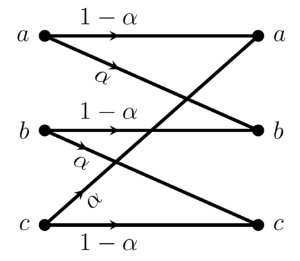
\includegraphics[width=\columnwidth]{./figs/figure1.png}
\label{Fig:1}
\end{figure}
\solution

\begin{tabular}{|c|c|c|} \hline
Variable & Description & Value\\\hline
$X$ & Input variable & $X = \cbrak{0,1,2}$\\\hline
$Y$ & Output variable & $Y = \cbrak{0,1,2}$\\\hline
$C$ & Channel Capacity & $C$\\\hline
$I$ & Mutual Information & $I$ \\\hline
$H$ & Entropy & $H$ \\\hline
\end{tabular}
\begin{align}
C &=\text{max}_{p\brak{X,Y}} I\brak{X,Y}\\
I\brak{X,Y} &= \sum_{x,y}p\brak{x,y}\log_2\frac{p\brak{x,y}}{p\brak{x}p\brak{y}}\\
&= \sum_{x,y}p\brak{x,y}\log_2\frac{p\brak{\left.{y}|\right.{x}}}{p\brak{y}}\\
&=-\sum_{x,y}p\brak{x,y}\log_2p\brak{y}+\sum_{x,y}p\brak{x,y}\log_2p\brak{\left.{y}|\right.{x}}\\
&=-\sum_{y}p\brak{y}\log_2p\brak{y}-\brak{-\sum_{x,y}p\brak{x,y}\log_2p\brak{\left.{y}|\right.{x}}}\\
&= H\brak{Y} - H\brak{\left.{Y}|\right.{X}}\label{eq:1}
\end{align}
Now,
\begin{align}
p_Y(0) &= p_Y(1) = p_Y(2) =\frac{1}{3}\\
H\brak{Y} &= - \sum_{y=0}^2p_Y\brak{y} \log_2p_Y\brak{y}\\
&= -\frac{1}{3}\log_2\frac{1}{3} \times 3\\
&= \log_23\label{eq:2}\\
H\brak{\left.{Y}|\right.{X}} &= -\sum_{x=0}^2 \sum_{y=0}^2p_X\brak{x}p_{\left.{Y}|\right.{X}}\brak{{\left.{y}|\right.{x}}}\log_2\brak{p_{\left.{Y}|\right.{X}}\brak{{\left.{y}|\right.{x}}}}\\
&=-\sum_{x=0}^2p_X\brak{x}\sum_{y=0}^2p_{Y}\brak{{\left.{y}|\right.{X}}}\log_2\brak{p_{Y}\brak{{\left.{y}|\right.{X}}}}\\
&=-3\times\frac{1}{3}\brak{\alpha\log_2\alpha+\brak{1-\alpha}\log_2\brak{1-\alpha}}\label{eq:3}
\end{align}
Using \eqref{eq:2} and \eqref{eq:3} in \eqref{eq:1}
\begin{align}
I\brak{X,Y}&= \log_23 + \alpha\log_2\alpha+\brak{1-\alpha}\log_2\brak{1-\alpha}\\
\implies \frac{d}{d\alpha}I\brak{X,Y} &= \brak{\log_2 \alpha - \log_2\brak{1-\alpha}}
\end{align}
For maxima or minima $\frac{d}{d\alpha}I\brak{X,Y} = 0$
\begin{align}
\log_2 \alpha - \log_2\brak{1-\alpha} &= 0\\
\alpha &= \frac{1}{2}\\
\frac{d^2}{d\alpha^2}I\brak{X,Y} &= \frac{1}{\log 2}\brak{\frac{1}{\alpha} + \frac{1}{1-\alpha}}\\
\left.{\frac{d^2}{d\alpha^2}I\brak{X,Y}}|_{\alpha = \frac{1}{2}}\right. &= \frac{4}{\log 2} \\
&\geq 0
\end{align}
At $\alpha = \frac{1}{2}, I\brak{X,Y}$ is minimum\\
\begin{figure}[!ht]
\centering
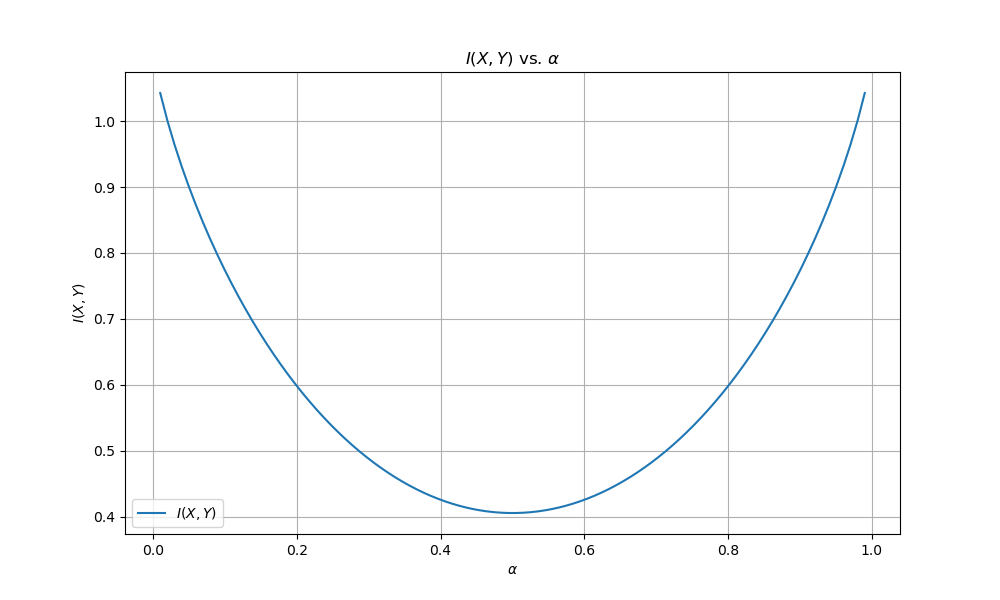
\includegraphics[width=\columnwidth]{./figs/figure2.png}
\label{Fig:2}
\end{figure}
As $I\brak{X,Y}$ is maximum at $\alpha = 0,1$\\
But $\alpha \in \sbrak{0.25,1}$, 
\begin{align}
\alpha = 1
\end{align}
\end{document}


